\section{Observability and controllability}

Let's consider the system described by:
\[\begin{cases} \mathbf{x}(t+1)=\mathbf{Fx}(t)+\mathbf{G}u(t) \\ y(t)=\mathbf{Hx}(t) \end{cases}\]
\begin{definition}[\textit{Fully observable}]
    A system is fully observable from the output $y(t)$ if and only if its observability matrix, denoted as $\mathbf{O}$, is full rank, meaning its rank equals the number of states $n$.
\end{definition}
The observability matrix is defined as: 
\[\mathbf{O}=\begin{bmatrix} \mathbf{H} \\ \mathbf{HF} \\ \mathbf{HF}^2 \\ \vdots \\ \mathbf{HF}^{n-1} \end{bmatrix}\]
Observability, which solely depends on $\mathbf{F}$ and $\mathbf{H}$, indicates that by observing the output $y(t)$, we can deduce the behavior of the system's state $\mathbf{x}(t)$. 

\begin{definition}[\textit{Fully controllable}]
    A system is fully controllable (or reachable) from the input $u(t)$ if and only if its controllability matrix, denoted as $\mathbf{R}$, is full rank, also equal to the number of states $n$.
\end{definition}
The reachability matrix is defined as: 
\[\mathbf{R}=\begin{bmatrix} \mathbf{G} & \mathbf{FG} & \mathbf{F}^2\mathbf{G} & \cdots & \mathbf{F}^{n-1}\mathbf{G} \end{bmatrix}\]
Controllability, which solely relies on $\mathbf{F}$ and $\mathbf{G}$, implies that by manipulating the input $u(t)$, we can affect the behavior of the system's state $\mathbf{x}(t)$. 


Categorizing state-space representations based on observability and controllability yields four distinct subsystems:
\begin{itemize}
    \item \textit{Non-observable and controllable}: in this case, the system's internal states cannot be fully inferred from the output, and not all states can be influenced by the input.
    \item \textit{Observable and non-controllable}: here, the system's states can be fully inferred from the output, but not all states can be influenced by the input.
    \item \textit{Observable and controllable}: this scenario indicates that both full observability and controllability are present, meaning all states can be inferred from the output and influenced by the input.
    \item \textit{Non-observable and non-controllable}: in this situation, neither full observability nor controllability exists. 
        The internal states cannot be fully inferred from the output, and not all states can be influenced by the input.
\end{itemize}
\begin{figure}[H]
    \centering
    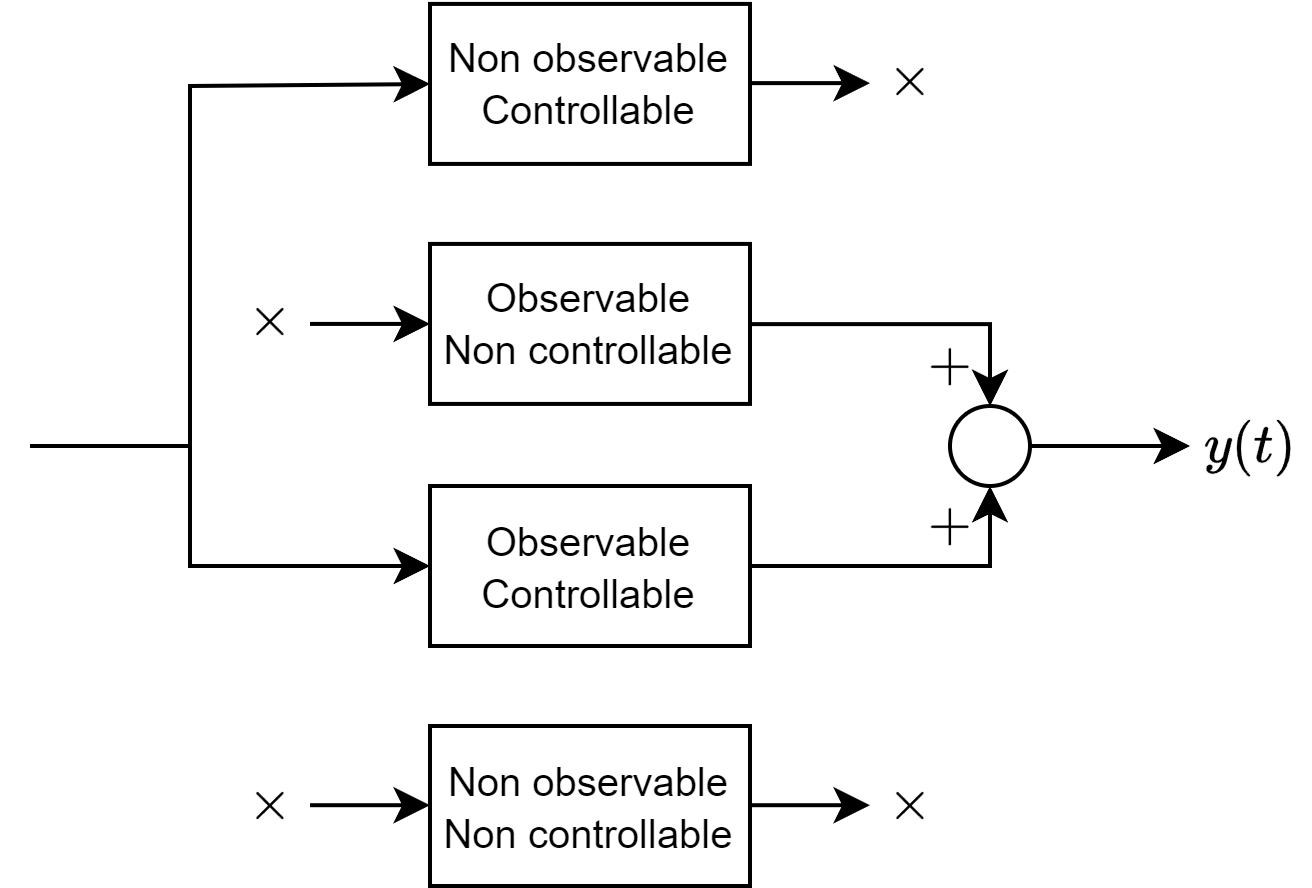
\includegraphics[width=0.5\linewidth]{images/subblock.png}
    \caption{State space subsystems}
\end{figure}
When representing these subsystems externally using a transfer function, only the observable and controllable parts of the system can be captured. 
The other subsystems, which lack either observability or controllability or both, remain hidden from the input and output perspective. 
Thus, the transfer function representation provides insight only into the observable and controllable aspects of the system.

\subsection{Hankel matrix}
The Hankel matrix of order $n$ is a square matrix constructed from the impulse response representation.
It starts from the impulse at time one (excluding zero), and each counter-diagonal contains responses from the same time instant. 
Mathematically, it's defined as:
\[\mathbf{H}_n=\begin{bmatrix} \omega(1) & \omega(2) & \omega(3) & \cdots & \omega(n) \\ \omega(2) & \omega(3) & \omega(4) & \cdots & \omega(n+1) \\ \omega(3) & \omega(4) & \omega(5) & \cdots & \omega(n+2) \\ \vdots & \vdots  & \vdots  & \vdots  & \vdots  \\ \omega(n) & \omega(n+1) & \omega(n+2) & \cdots & \omega(2n-1) \end{bmatrix}\]
Given the transformation from transfer function to impulse response representations:
\[\omega(t)=\mathbf{HF}^{t-1}\mathbf{G} \qquad \text{if } t \geq 1\]
We can rewrite the Hankel matrix as:
\[\mathbf{H}_n=\begin{bmatrix} \mathbf{HG} & \mathbf{HFG} & \mathbf{HF}^2\mathbf{G}  & \cdots & \mathbf{HF}^{n-1}\mathbf{G} \\ \mathbf{HFG} & \mathbf{HF}^2\mathbf{G} & \mathbf{HF}^3\mathbf{G}  & \cdots & \mathbf{HF}^{n}\mathbf{G} \\ \mathbf{HF}^2\mathbf{G} & \mathbf{HF}^3\mathbf{G} & \mathbf{HF}^4\mathbf{G}  & \cdots & \mathbf{HF}^{n+1}\mathbf{G} \\ \vdots & \vdots  & \vdots  & \ddots  & \vdots  \\ \mathbf{HF}^{n-1}\mathbf{G} & \mathbf{HF}^{n}\mathbf{G} & \mathbf{HF}^{n+1}\mathbf{G}  & \cdots & \mathbf{HF}^{2n+2}\mathbf{G} \end{bmatrix}=\begin{bmatrix} \mathbf{H} \\ \mathbf{HF} \\ \mathbf{HF}^2 \\ \vdots \\ \mathbf{HF}^{n-1} \end{bmatrix} \cdot \begin{bmatrix} \mathbf{G} \\ \mathbf{FG} \\ \mathbf{F}^2\mathbf{G} \\ \vdots \\ \mathbf{F}^{n-1}\mathbf{G} \end{bmatrix}^T\]
Therefore, the Hankel matrix is the outer product of the observability and controllability matrices. 